\chapter{Modellazione e sviluppo dell'ontologia}
Durante lo sviluppo dell'ontologia si è cercato il più possibile di integrare le ontologie già esistenti citate, in modo da non dover ripetere la modellazione di classi e proprietà già definite e rendere tutto più consistente.\\

Tutte le classi che classi che presentano una equivalenza sono state definite come \textbf{Defined Class} ovvero una classe che ha almeno una condizione necessaria e sufficente (all'interno di Protègè queste classi vengono chiamate Equivalent Class). Nella pratica stiamo dicendo che se un individuo è un membro della classe A deve soddisfare le condizioni ed inoltre possiamo dire che se un individuo soddisfa queste condizioni allora deve essere un membro della classe A. Questa scelta è stata fatta per aiutare il reasoner a inferire meglio le classi (si veda \cite{definedclass}).

\section{Big Data Technology}
La classe \textbf{Big Data Technololgy} è l'entità principale dell'ontologia, la quale è una generificazione delle tre sottoclassi \textbf{Big Data Service}, \textbf{Big Data Tool} e \textbf{Programming Language}. L'importanza di questa classe risiede nel fatto che ogni specializzazione di essa deriva da essa stessa e quindi ognuna delle sottoclassi presenterà una equivalenza diretta alla classe madre.\\

Alcune delle proprietà (numeriche e non) sono applicabili a tutte le entità di tipo Big Data Technology. Alcune di queste però, sono necessarie affinchè una tecnologia si specializzi in una sottoclasse. Nelle sezioni seguenti anallizzeremo più approfonditamente alcune delle classi più importanti dell'ontologia.
\newpage
\subsection{Big Data Tool}
Una software specifico per i Big Data è definito \textbf{Big Data Tool}. Attualmente sono stati modellati solo alcuni tra i molteplici tool Big Data, come si evince dalla figura \ref{fig:bdtool_graph}.

\begin{figure}[H]
    \centering
    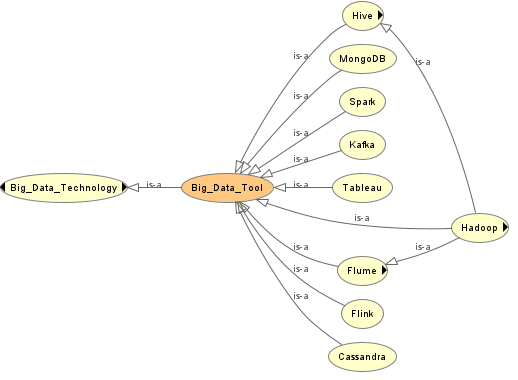
\includegraphics[width=12cm]{docs/images/bdtoolowlviz.png}
    \caption{Gerarchia dei Big Data Tool creato su Protègè tramite il plugin OWLViz.}
    \label{fig:bdtool_graph}
\end{figure}

Una tecnologia Big Data per essere definita Tool dovrà rispettare alcune condizioni necessarie e sufficienti. Per ogni Tool sono presenti:
\begin{verbatim}
Big_Data_Technology
    and (supportsWith some Programming_Language)
    and (hasAverageSize exactly 1 xsd:float)
    and (hasDifficultyLevel exactly 1 xsd:int)
    and (hasEndOfSupportDate exactly 1 xsd:dateTime)
    and (hasLearningCurve exactly 1 xsd:int)
    and (hasVersion exactly 1 xsd:string)
\end{verbatim}

\newpage

Come si può vedere nell'esempio di istanza in figura \ref{fig:cassandra_graph} tutte le condizioni affinchè una tecnologia venga classificata come tool sono state soddisfatte ed è inoltre presente un'altra istanza (\textit{Cassandra\_V.2.7.9}) che presenta una retrocompatibilità con l'istanza in questione: questa informazione è resa possibile dal reasoner e dalla proprietà inversa \textit{isCompatibleWith}.

\begin{figure}[H]
    \centering
    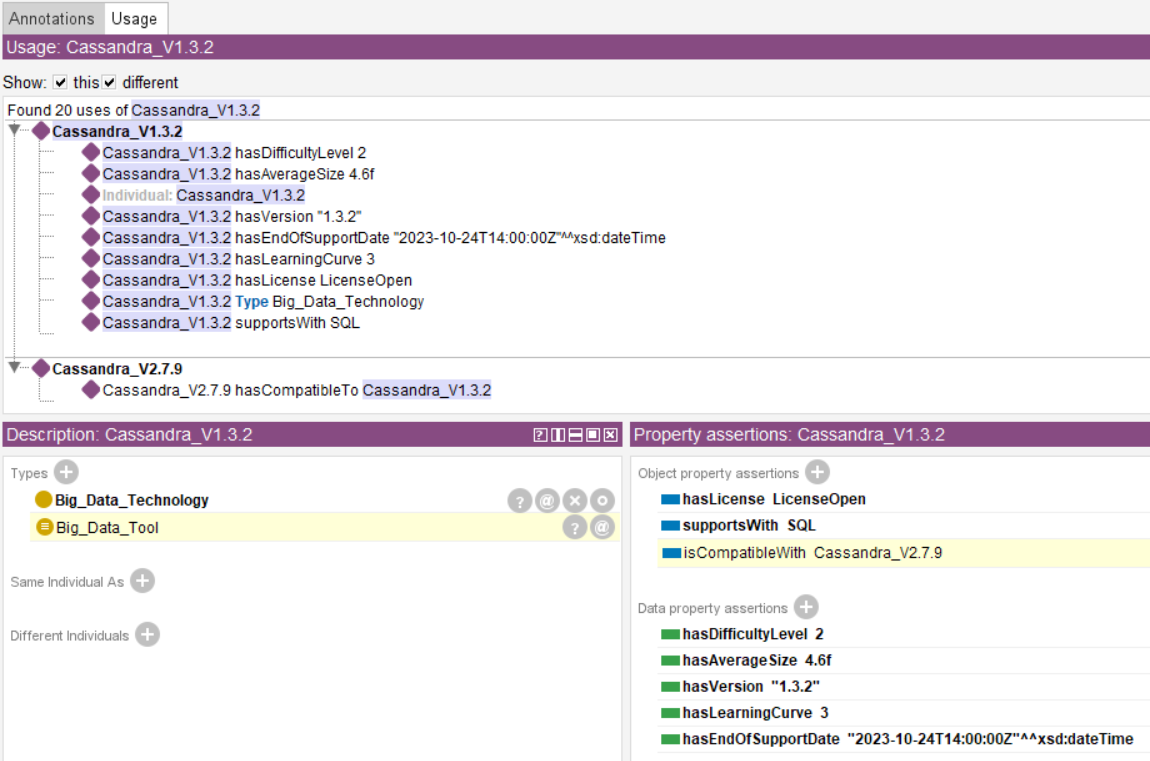
\includegraphics[width=15cm]{docs/images/cassandraex.PNG}
    \caption{Esempio di istanza di Big Data Technology classificata come Big Data Tool dal reasoner di Protègè, Pellet.}
    \label{fig:cassandra_graph}
\end{figure}

Infine, è stato modellato anche il concetto di impiego di un tool da parte di un altro. L'esempio migliore che si possa fare è Hadoop che consiste di tante tecnologie (es. Flume). Questa peculiarità è modellata con l'object property chiamata \textit{usesTechnology}.
\newpage
\subsection{Big Data Service}
Un servizio Big Data è un'offerta o una piattaforma fornita da un fornitore di servizi che consente alle organizzazioni di gestire, analizzare e sfruttare grandi volumi di dati in modo efficiente e scalabile. Tipicamente questi servizi offrono delle soluzioni che consentono l'utilizzo di software all'interno dei lori sistemi. Come si vede dalla figura \ref{fig:bdservice_graph}, l'ontologia prevede due tipi di soluzioni: quella cloud e quella on-premises.

\begin{figure}[H]
    \centering
    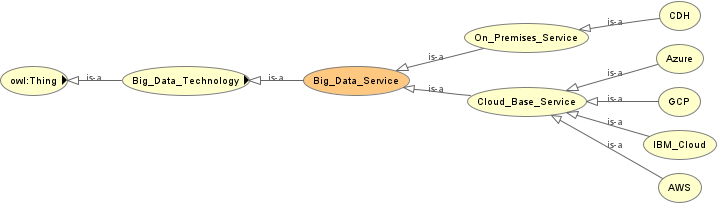
\includegraphics[width=12cm]{docs/images/bdserviceowlviz.png}
    \caption{Gerarchia dei Big Data Service creato su Protègè tramite il plugin OWLViz.}
    \label{fig:bdservice_graph}
\end{figure}

Come per i tool, anche i servizi sono un'estensione delle tecnologie big data e quindi presentano una condizione necessaria e sufficente:
\begin{verbatim}
Big_Data_Technology
 and (supportsWith some Big_Data_Tool)
 and (hasPlatform some Company)
 and (hasAverageCost exactly 1 xsd:float)
 and (hasDifficultyLevel exactly 1 xsd:int)
 and (hasLearningCurve exactly 1 xsd:int)
 and (hasVersion exactly 1 xsd:string)
\end{verbatim}

Il fornitore che offre un servizio o che dà la possibilità di installare il proprio servizio in locale è una proprietà fondamentale dei servizi Big Data, come si evince dalla figure \ref{fig:awsex_graph}.

\begin{figure}[H]
    \centering
    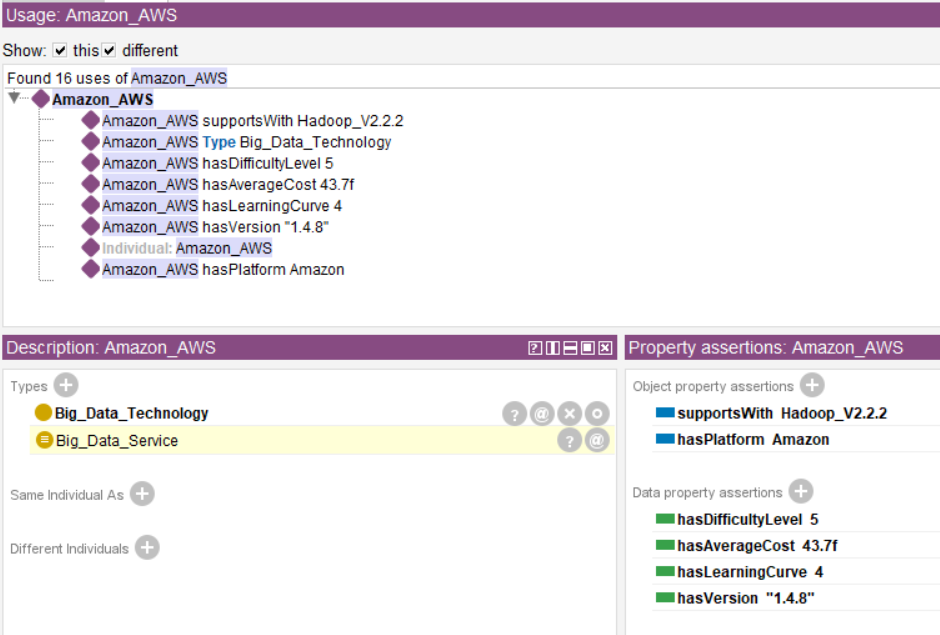
\includegraphics[width=15cm]{docs/images/awsex.PNG}
    \caption{Esempio di istanza di Big Data Technology classificata come Big Data Service dal reasoner di Protègè, Pellet.}
    \label{fig:awsex_graph}
\end{figure}

\section{Data Science Process}
Il Data Science Process è una sequenza organizzata di attività che mira a estrarre valore e conoscenza dai dati: questa classe rappresenta la macro-attività di questo processo.\\

In generale, questo processo può variare leggermente a seconda del contesto e degli obiettivi specifici, ma in questo progetto ci basiamo sulla definizione data in \cite{naous2017analytics} e \cite{BDOnto}. La sequenza di azioni svolte durante un progetto legato al mondo della Data Science, comprende degli step predefiniti (es. Data Analysis) che a loro volta comprendono delle operazioni che vengono svolte. Le operazioni che vengono svolte tendono ad essere mappate ad uno step della sequenza. Ad esempio, l'operazione di Data Gathering viene svolta nello step di Data Provision. Partendo quindi dalla classe madre, Data Science Process, troviamo due sottoclassi principali, General Steps e Operation, come si evince dalla figura \ref{fig:dataproc}.
\begin{figure}[H]
    \centering
    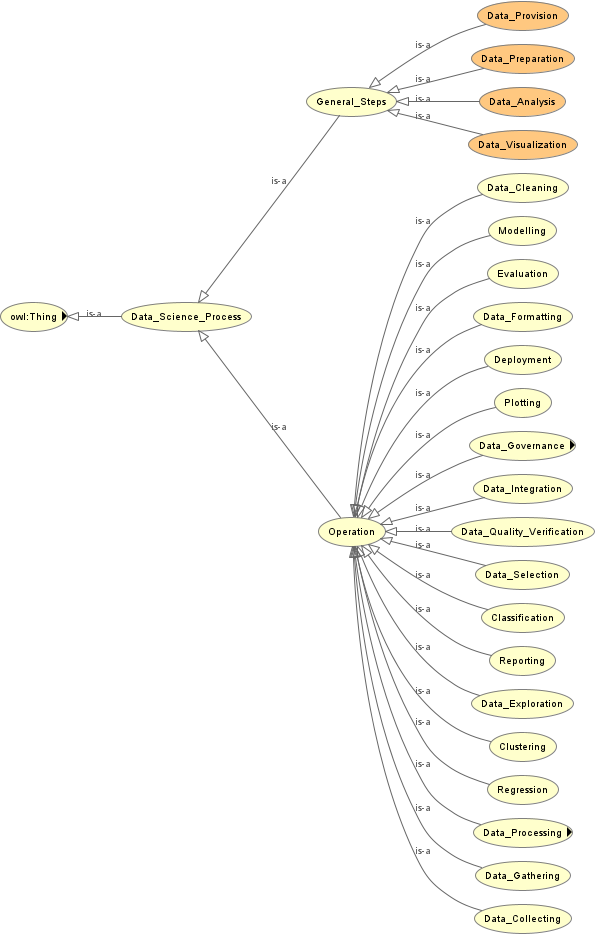
\includegraphics[height=13cm]{docs/images/dataprocowlviz.png}
    \caption{Gerarchia del Data Science Process, con una vista sulla due sottoclassi principali: General Steps e Operation}
    \label{fig:dataproc}
\end{figure}
\subsection{General Steps}
Per descrivere le operazioni di un Data Science Process, è stata creata la classe General Steps. Il flow, e quindi l'ordine, di queste operazioni è caratterizzato dalla proprietà \textit{directlyFollowedBy} che, come si può facilmente intuire, regola lo step successivo ad uno dato. Troviamo quattro step, Data Provision, Data Preparation, Data Analysis e Data Visualization,il cui ordine è mostrato in figura \ref{fig:hasSubclass}, che presenta anche una legenda del grafo.
\begin{figure}[H]
    \centering
    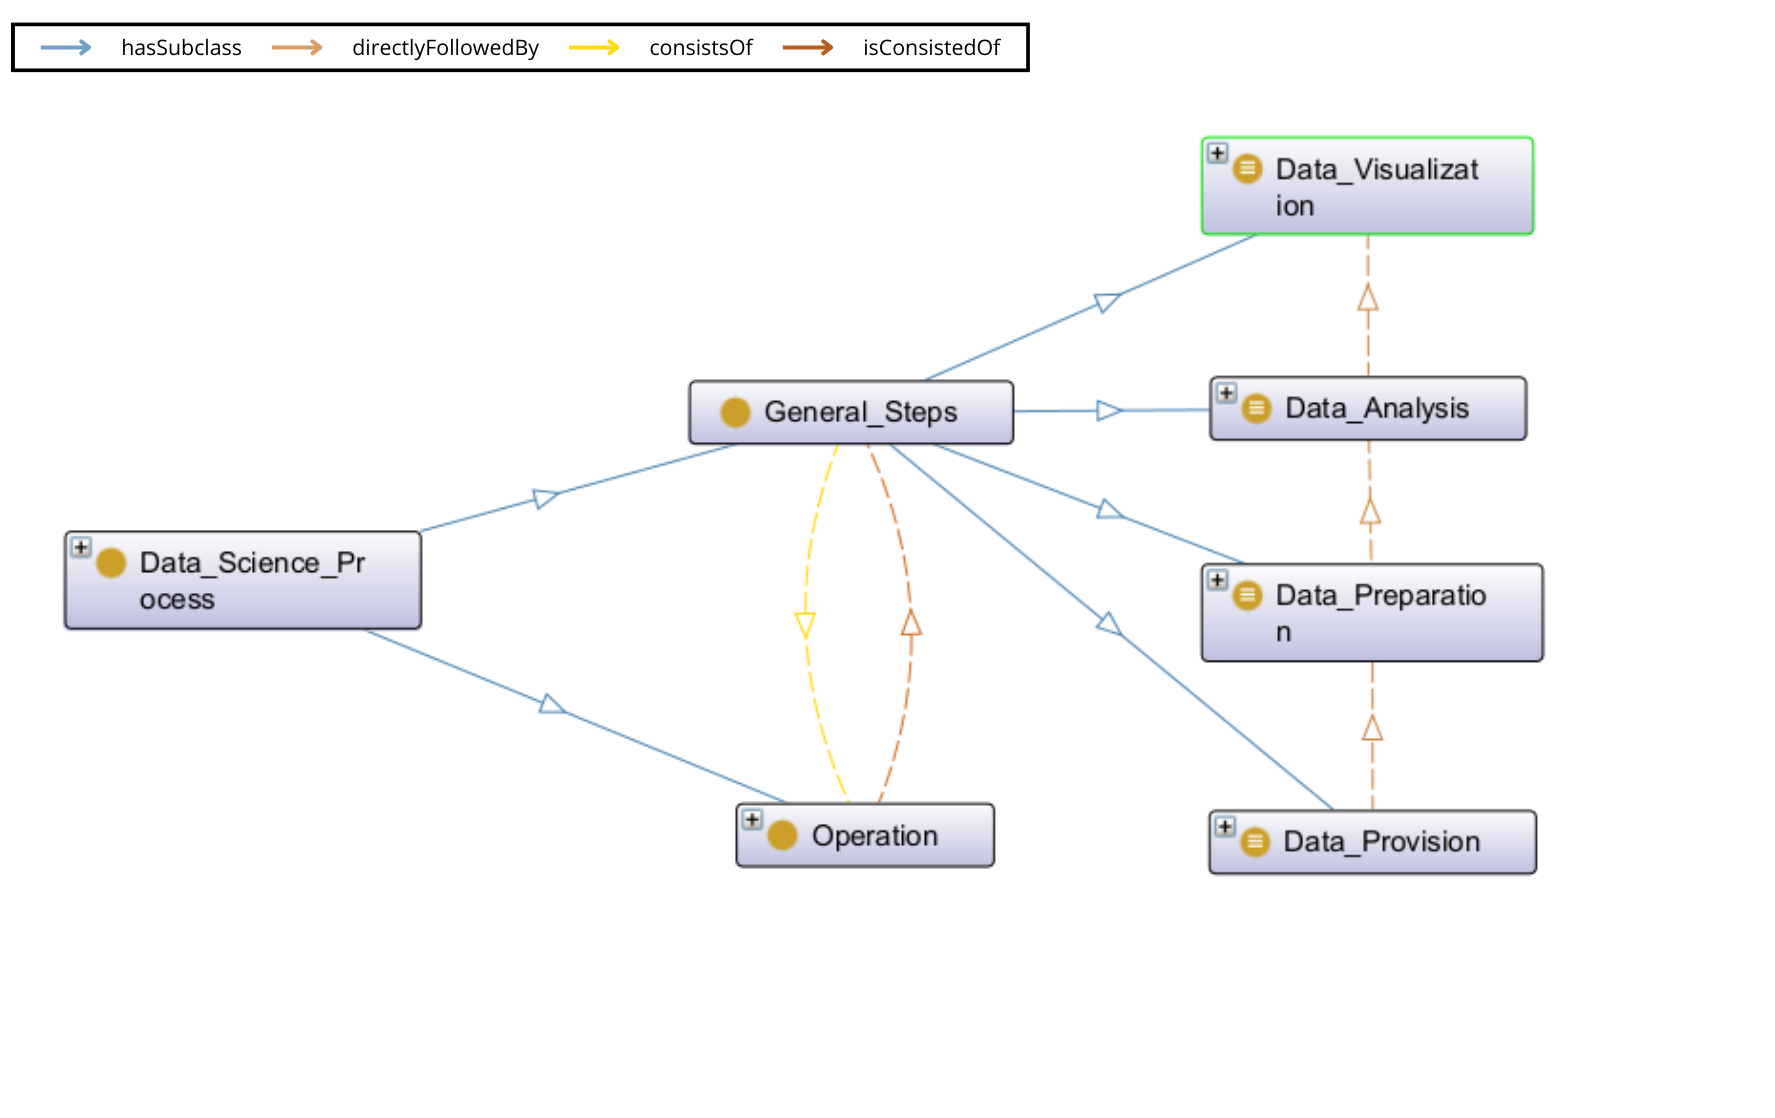
\includegraphics[width=12cm]{docs/images/hasSubclass.png}
    \caption{Ordinamento degli step all'interno di un processo di Data Science, rappresentato graficamente dal plugin OntoGraf all'interno di Protègè.}
    \label{fig:hasSubclass}
\end{figure}

Ogni specifico step è sottoclasse di General Steps, con obiettivi e rappresentazioni diversi. Ad esempio, la fase di Data Analysis punta a esaminare ed interpretare i dati mentre quella di Data Visualization si occuperà per lo più della interpretabilità dei dati. È intuibile quindi che ogni fase avrà operazioni diverse: questa relazione è modellata dalla proprietà \textit{consistsOf} (e dalla sua inversa \textit{isConsistedOf}). Si prenda come esempio la classe \textit{Data Analysis} e la sua descrizione mostrata in figura \ref{fig:data_anal}.
\begin{figure}[H]
    \centering
    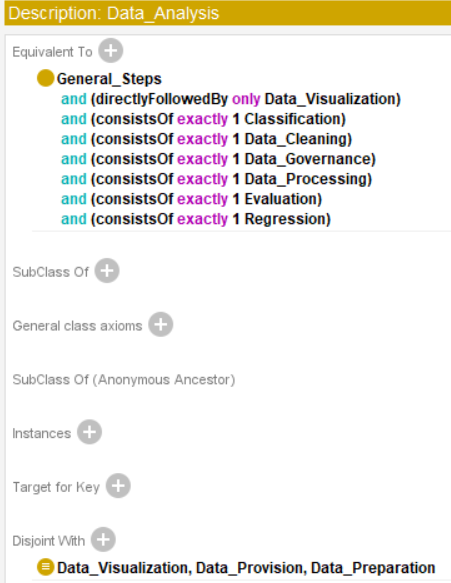
\includegraphics[height=6.3cm]{docs/images/datanaldesc.PNG}
    \caption{Descrizione della classe Data Analysis.}
    \label{fig:data_anal}
\end{figure}

Siccome ogni specifico step può essere visto come uno step generico che comprende determinate operazioni, è stato deciso di modellare questa peculiarità all'interno di una equivalenza per ognuno dei singoli step. Prendiamo il caso della classe \textit{Data Preparation}:

\begin{verbatim}
General_Steps
 and (directlyFollowedBy only Data_Analysis)
 and (consistsOf exactly 1 Clustering)
 and (consistsOf exactly 1 Data_Exploration)
 and (consistsOf exactly 1 Data_Formatting)
 and (consistsOf exactly 1 Data_Governance)
 and (consistsOf exactly 1 Data_Quality_Verification)
 \end{verbatim}

Si noti come, per sua natura, l'operazione di \textit{Data Governance} è inclusa in tutte le fasi del processo: l'attenzione alla privcacy e alla sicurezza del dato, soprattutto se sensibile, è un aspetto da non sottovalutare lungo tutta la durata del progetto.

\section{Operation}
Mentre la classe \textit{General Steps} descrive l'andamento del processo, la classe \textbf{Operation} contiene diverse operazioni, che sono spesso effettuate in una specifica fase. Alla lista iniziale (definita in \cite{BDOnto}) di operazioni ne sono state aggiunte alcune come la \textbf{Data Governance} e la \textbf{Data Processing}.\\

Ogni operazioni è tanto legata ai singoli step quanto alle tecnologie che sfruttano per arrivare al loro goal. Troviamo quindi la proprietà chiamata \textit{hasParticipant} che lega una operazione ad una o più tecnologie. Chiaramente un compito può essere svolto in egual maniera da tanti tool, sarà poi quindi l'utente finale a scegliere quale tool utilizzare per un dato compito. Ogni sottoclasse di Operation avrà quindi dei "partecipanti" al proprio stadio, come ad esempio la classe \textbf{Data Processing} mostrata in figura \ref{fig:dataprocdesc}, si lega a tre tool: Hadoop, Flink e Spark.

\begin{figure}[H]
    \centering
    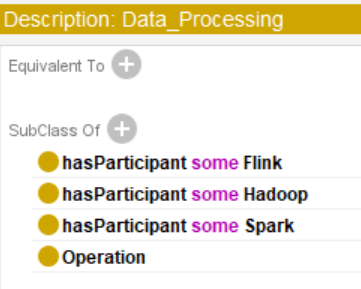
\includegraphics{docs/images/dataprocdesc.PNG}
    \caption{Descrizione di una sottoclasse di Operation: in questo caso Data Processing e le sue relazioni.}
    \label{fig:dataprocdesc}
\end{figure}

Nel contesto dei Big Data, un dominio estramemente frizzante in cui vengono definiti nuovi concetti giorno dopo giorno, è estramemnte probabile che estensioni e approfondimenti delle operazioni qui definite vengano aggiunte. In tale caso, la classe Operation si presta bene a nuove estensioni o migliorie.


\section{Server}
L'hardware rappresenta la "parte tangibile" di un sistema informatico o di un dispositivo elettronico. Un hardware può essere chiaramente anche il sistema informatico stesso come un telefono o un laptop. Le componenti hardware di tali sistemi sono gli stessi presenti in un computer, nodo o server, più in generale, che ci permettono di elaborare grandi quantità di dati. Da questa analisi è nata la classe \textbf{Server}, una classe che estende l'ontologia Hardware Ontology \cite{Hardware_Ontology} e che rappresenta appunto un una  macchina in grado di elaborare, gestire ed archiviare grandi volumi di dati. Di base, questi calcolatori sono usati in combinazione con loro simili. Inoltre, le specifiche tecniche di questi server sono paragonabili a computer di fascia alta.

\begin{figure}[H]
    \centering
    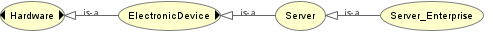
\includegraphics[width=12cm]{docs/images/bdhwowlviz.png}
    \caption{Gerarchia dalla classe Hardware creata su Protègè tramite il plugin OWLViz.}
    \label{fig:bdhw_graph}
\end{figure}

Le compomenti fisiche come la CPU, la RAM eccetera eccetera, danno vita ai server. Volendo modellare quest'ultimo concetto, ci siamo trovati dinanzi alla necessità di dover progettare a cascata tutti i concetti che compongono questi server (come detto, CPU, RAM, ecc.). L'impiego dell'ontologia Hardware Ontology \cite{Hardware_Ontology} è stato di estrema importanza: ci ha permesso di riutilizzare classi già da essa definite.\\
 
I server che tipicamente si impiegano sui progetti di Data Science o Big Data si definiscono in Server Commodity, ovvero dei server meno performanti e affidabili; per brevità questa classe è stata decisa di chiamarla più semplicemente \textbf{Server}. Quei server più affidabili e con prestazioni migliori vengono definiti \textbf{Server Enterprise}. Inizialmente volevamo rendere una Defined Class anche questa classe. Il solo OWL però non permetteva la modellazione ciò che avremmo voluto fare:  vedremo nel successivo capitolo, in particolare in \ref{sec:swrl}, come il reasoner ed in particolare le regole \textbf{SWRL} ci hanno aiutato in questo compito.